\documentclass[11pt]{article}

\usepackage[a4paper,margin=1in]{geometry}
\usepackage[T1]{fontenc}
\usepackage[utf8]{inputenc}
\usepackage{lmodern}
\usepackage{microtype}
\usepackage{amsmath,amssymb,amsthm,mathtools}
\usepackage{booktabs}
\usepackage{graphicx}
\usepackage{float}
\usepackage{placeins}
\usepackage{enumitem}
\usepackage[numbers,sort&compress]{natbib}
\usepackage{xcolor}
\usepackage{xurl}
\usepackage[colorlinks=true,linkcolor=blue!55!black,citecolor=blue!55!black,urlcolor=blue!55!black]{hyperref}
\usepackage[nameinlink,noabbrev]{cleveref}

\setlength{\parindent}{1.4em}
\setlength{\parskip}{0.15em}
\setlist{itemsep=0.25em,topsep=0.35em}

\newtheorem{theorem}{Theorem}[section]
\newtheorem{proposition}[theorem]{Proposition}
\newtheorem{lemma}[theorem]{Lemma}
\newtheorem{corollary}[theorem]{Corollary}
\theoremstyle{definition}
\newtheorem{definition}[theorem]{Definition}
\newtheorem{conjecture}[theorem]{Conjecture}
\theoremstyle{remark}
\newtheorem{remark}[theorem]{Remark}

\newcommand{\R}{\mathbb R}
\newcommand{\C}{\mathbb C}
\newcommand{\uc}{u_{\mathrm c}}
\newcommand{\cK}{\mathcal K}
\newcommand{\cP}{\mathcal P}
\newcommand{\cL}{\mathcal L}
\newcommand{\cT}{\mathcal T}
\newcommand{\cS}{\mathcal S}
\newcommand{\cA}{\mathcal A}
\newcommand{\cB}{\mathcal B}
\newcommand{\cC}{\mathcal C}
\newcommand{\cG}{\mathcal G}
\newcommand{\Id}{\mathrm I}
\newcommand{\Dettwo}{\operatorname{Det}_2}

\title{\textbf{Parity-Extracted Bulk Scattering}\\
\textbf{at a Quadratic Band-Merging Map:}\\[0.35em]
\large Exact Endpoint Poles, Resonance-Cloud Necessity,\\
and Geometric Finite-Section Scaling}
\author{Liang Wang\\
\small School of Artificial Intelligence and Automation,\\[-0.2em]
\small Huazhong University of Science and Technology, Wuhan 430074, P.R. China\\
\small \texttt{wangliang.f@gmail.com}}
\date{July 2026}

\begin{document}

\maketitle

\begin{abstract}
At the algebraic band-merging parameter of $f_u(x)=1-u x^2$, the
zero-noise Perron operator has the peripheral pair $1,-1$.  Gaussian noise
moves the parity mode to a resonance $\lambda_-(\sigma)>-1$.  After removing
both peripheral factors, every fixed Taylor coefficient of the noisy
Hilbert--Schmidt determinant has a deterministic limit.  The unresolved
question is whether these coefficients assemble into a genuine bulk
determinant limit.

We first identify the target exactly.  Let $S=f^2$ on one mixing component,
let $E_{1,n}$ be the even $\beta=1$ trace of its analytic circle lift, and put
$a_n=\lambda^{-n}$, where $\lambda=2u_{\mathrm c}(u_{\mathrm c}-1)$.  The
physical flat trace, including the orbifold branch point, satisfies
\[
 P_{2n}=2E_{1,n}
 -\frac{2a_n}{1+a_n}
 -\frac{a_n^2}{1-a_n^2}.
\]
The validated reduced-sector bound $r_1<1/3$ therefore yields the sharp law
\[
 P_{2n}=2-2\lambda^{-n}+\lambda^{-2n}+O(3^{-n}).
\]
Exponentiating the exact trace identity gives a convergent endpoint
$q$-product factorization of the parity-centered determinant:
\[
 \boxed{
 \widehat D_{0,\mathrm{bulk},2}(z)
 =\frac{\cG(z)}{1-z^2/\lambda}},
 \qquad
 \cG(z)\ne0\quad(|z|<\lambda).
\]
Thus $z=\pm\sqrt\lambda$ are genuine simple poles.  In particular, the
entire noisy bulk determinants cannot converge locally uniformly on any disk
containing either pole.  The negative leading moments also rule out every
fixed finite-resonance realization of the deterministic edge: a growing
resonance cloud is necessary.

The canonical finite section of the pole is
\[
 \Pi_N(q)=1+q+\cdots+q^N=\frac{1-q^{N+1}}{1-q},
 \qquad q=z^2/\lambda.
\]
It has $2N$ reciprocal resonances at radius $\lambda^{-1/2}$ and phases
$\pm k\pi/(N+1)$, and its radially scaled limit is
$(e^s-1)/s$.  Sparse Gaussian computations down to $\sigma=10^{-4}$ resolve
an outer cloud of fourteen eigenvalues.  Their phase root-mean-square error
from the $N=7$ geometric grid is $0.01124$ radians, while their mean radius
moves toward $\lambda^{-1/2}=0.7718445\ldots$.  The radially centered cloud
factor follows the finite geometric model.  These spectral-cloud statements
are floating-point evidence and motivate a precise scattering conjecture;
the trace reconstruction, endpoint poles, normal-family obstruction, and
finite-section model are analytic results.
\end{abstract}

\noindent\textbf{Keywords:} transfer operator; regularized determinant;
flat trace; resonance cloud; finite-section scattering; quadratic map;
small noise; spectral condensation; boundary layer.

\medskip
\noindent\textbf{MSC 2020:} 37E05; 37D25; 47A55; 47B10; 65P30.

\section{Introduction}
\label{sec:introduction}

Small noise can approximate every fixed periodic coefficient and still fail
to approximate the analytic object assembled from all periods.  This is the
central difficulty in taking a simultaneous small-noise/long-cycle limit.
For the quadratic band-merging map, the difficulty is visible but unusually
structured.  Deterministic dynamics has two cyclic components, hence a
parity eigenvalue $-1$.  Positive Gaussian noise makes the Markov operator
strongly mixing and turns that eigenvalue into a long-lived negative
resonance.

The preceding sequence of papers separated the relevant mechanisms.  Exact
Markov counts and fixed-length Gaussian localization produced the physical
flat traces and exposed a logarithmic localization horizon
\citep{WangLongCycle2026}.  Collet--Eckmann weighted-zeta theory proved an
unconditional parity-centered trace gap \citep{WangFlatTrace2026}.  An
analytic circle lift then isolated the postcritical factors, and a validated
Wiener--Taylor calculation proved their noncancellation
\citep{WangPostcritical2026,WangValidatedGap2026}.  Finally, coupled
critical-value boundary layers corrected the parity splitting to
\begin{equation}\label{eq:parity-law-intro}
 1+\lambda_-(\sigma)
 =C_*\sqrt\sigma+o(\sqrt\sigma).
\end{equation}
This boundary-layer law was established in \citet{WangBoundaryLayer2026}.

After these steps, the finite-noise parity-extracted determinant has no
remaining ambiguous peripheral factor.  For each fixed $m\ge2$, its trace
coefficient converges to the deterministic parity-centered flat trace.  It
is tempting to infer convergence of the whole determinant.  The first result
of this paper is that this temptation is only locally correct: the exact
deterministic target is meromorphic, not entire, and its first singularities
are two endpoint poles at $\pm\sqrt\lambda$.

The poles explain the numerical spectrum.  A finite-noise determinant is
entire, so it cannot converge normally through a deterministic pole.  As the
noise decreases, more bulk eigenvalues gather near the reciprocal circle
$|\mu|=\lambda^{-1/2}$.  Their phases are close to the roots-of-unity grid
generated by a geometric polynomial.  The cloud is therefore not an
arbitrary collection of fitted eigenvalues: it survives a spatial-resolution
audit and matches the only canonical finite section considered here.  The
claim that it is the actual finite-noise pole-resolution mechanism remains
the scattering conjecture formulated below.

\subsection*{Main results and status}

\begin{enumerate}[label=\textbf{R\arabic*.},leftmargin=3.2em]
 \item The physical component flat trace is reconstructed exactly from the
 even $\beta=1$ circle trace.  This is a new Lefschetz/orbifold identity,
 distinct from the earlier Perron-weight identity.

 \item Combining that identity with the validated reduced-sector bound gives
 \[
  P_{2n}=2-2\lambda^{-n}+\lambda^{-2n}+O(3^{-n}).
 \]

 \item The full physical determinant factors into one reduced Fredholm
 determinant and three explicit endpoint $q$-products.  After Perron/parity
 extraction,
 \[
  \widehat D_{0,\mathrm{bulk},2}(z)
  =\cG(z)/(1-z^2/\lambda),
  \qquad \cG\ne0\quad(|z|<\lambda).
 \]

 \item Coefficientwise noisy convergence is unconditional, but no locally
 uniform entire limit can cross $\pm\sqrt\lambda$.  This is a normal-family
 obstruction, not a numerical inference.

 \item The negative leading even moments cannot arise from any fixed finite
 multiset of limiting resonances.  A growing cloud or an infinite-dimensional
 spectral edge is mathematically necessary.

 \item The exact geometric pole section $\Pi_N$ has quantized reciprocal
 resonances and the scaled profile $(e^s-1)/s$.  This is an analytic model
 theorem.

 \item Sparse computations with as many as $204800$ states identify the
 effective degrees $3,3,4,5,5,6,7$ as $\sigma$ decreases from $10^{-2}$ to
 $10^{-4}$.  Agreement of the noisy cloud with the geometric model is an
 ordinary floating-point diagnostic.  The asymptotic noisy scattering law is
 stated as a conjecture and route map.
\end{enumerate}

\section{The deterministic and noisy objects}
\label{sec:setup}

Let $u=\uc$ be the root in $(1,2)$ of
\begin{equation}\label{eq:cubic}
 u^3-2u^2+2u-2=0,
\end{equation}
and set
\begin{equation}\label{eq:constants}
 r=\uc-1,
 \qquad
 \lambda=2\uc r.
\end{equation}
Then
\begin{equation}\label{eq:critical-orbit}
 0\longmapsto1\longmapsto-r\longmapsto r\longmapsto r,
\end{equation}
and
\begin{equation}\label{eq:numerical-constants}
 \lambda=1.678573510428322\ldots,
 \quad
 \sqrt\lambda=1.295597742522085\ldots,
 \quad
 \lambda^{-1/2}=0.771844506346038\ldots.
\end{equation}

Write $f(x)=1-\uc x^2$.  Every periodic point is repelling.  Its physical
flat trace is
\begin{equation}\label{eq:physical-trace}
 P_m=\sum_{f^mp=p}\frac1{|1-(f^m)'(p)|}.
\end{equation}
The deterministic parity-centered coefficients are
\begin{equation}\label{eq:centered-coefficients}
 c_m=P_m-1-(-1)^m.
\end{equation}
They define the second-regularized bulk germ
\begin{equation}\label{eq:deterministic-bulk}
 \widehat D_{0,\mathrm{bulk},2}(z)
 =\exp\left[-\sum_{m\ge2}\frac{c_mz^m}{m}\right].
\end{equation}

For $\sigma>0$, let $\cK_\sigma$ be the row-normalized Gaussian Markov
operator on $[-1,1]$.  It is Hilbert--Schmidt, with simple Perron root one and
simple real parity resonance $\lambda_-(\sigma)$.  Removing those two
eigenvalues from its second regularized determinant gives
\begin{align}
 D_{\sigma,\mathrm{bulk},2}(z)
 &=\prod_{\mu\in\operatorname{spec}_{\mathrm{bulk}}(\cK_\sigma)}
 (1-z\mu)e^{z\mu}
 \label{eq:noisy-product}\\
 &=\exp\left[-\sum_{m\ge2}\frac{c_{\sigma,m}z^m}{m}\right],
 \qquad
 c_{\sigma,m}=\operatorname{tr}\cK_\sigma^m-1-\lambda_-(\sigma)^m.
 \label{eq:noisy-traces}
\end{align}
For each fixed noise this is entire \citep{Simon2005}.

\subsection{The circle-lift input}

Let $S=f^2$ on the central component $[-r,r]$.  The cosine cover
\begin{equation}\label{eq:cosine-cover}
 \pi(\theta)=-r\cos\theta
\end{equation}
semiconjugates $S$ to an analytic expanding degree-two circle map $F$.
Let $E_{1,n}$ denote the flat trace of the even deck sector of the analytic
transfer operator with weight $(F')^{-1}$, and let $D_{1,+}$ be its Fredholm
determinant.  The Perron eigenvalue gives
\begin{equation}\label{eq:perron-deflation}
 D_{1,+}(w)=(1-w)\widetilde D_{1,+}(w),
 \qquad
 E_{1,n}=1+\operatorname{tr}(\cT_{1,0}^n).
\end{equation}

The validated result of \citet{WangValidatedGap2026} is
\begin{equation}\label{eq:validated-radius}
 r(\cT_{1,0})
 \le0.329642076293171<\frac13,
\end{equation}
and $\widetilde D_{1,+}$ is zero-free for
\begin{equation}\label{eq:certified-disk}
 |w|<R_{\mathrm{cert}}=3.0335933180\ldots>\lambda^2.
\end{equation}
This is a computer-assisted theorem based on directed Arb arithmetic.  We use
it as a proved input; no new interval calculation is claimed here.

\section{Exact reconstruction of the physical flat trace}
\label{sec:trace-reconstruction}

Define the physical component trace
\begin{equation}\label{eq:component-physical}
 p_n=\sum_{S^nx=x}\frac1{|1-(S^n)'(x)|}.
\end{equation}
The distinction between $p_n$ and the Perron-weight trace is concentrated at
the fixed-point denominator and at the branch endpoint $r$.

\begin{theorem}[Physical circle-to-interval reconstruction]
\label{thm:physical-reconstruction}
For every $n\ge1$, with $a_n=\lambda^{-n}$,
\begin{equation}\label{eq:component-reconstruction}
 \boxed{
 p_n=E_{1,n}-\frac{a_n}{1+a_n}.}
\end{equation}
Consequently the full-map traces are
\begin{align}
 P_{2n}
 &=2E_{1,n}
 -\frac{2a_n}{1+a_n}
 -\frac{a_n^2}{1-a_n^2},
 \label{eq:even-reconstruction}\\
 P_{2n+1}
 &=\frac{\lambda^{-(2n+1)}}{1+\lambda^{-(2n+1)}}.
 \label{eq:odd-reconstruction}
\end{align}
\end{theorem}

\begin{proof}
Let $x\ne r$ be fixed by $S^n$, and let its two circle lifts be
$\theta,-\theta$.  Put $a=D_n(\theta)^{-1}$, where
$D_n=(F^n)'$.  If $F^n\theta=\theta$, both lifts occur in the ordinary fixed
set.  Their combined contribution to the even $\beta=1$ sector is
\[
 \frac12\left(\frac a{1-a}+\frac a{1-a}\right)
 =\frac1{D_n-1}.
\]
The interval multiplier is positive and equals $D_n$, so this is exactly the
physical contribution in \eqref{eq:component-physical}.

If $F^n\theta=-\theta$, both lifts occur in the deck-twisted fixed set.  Their
even-sector contribution is
\[
 \frac12\left(\frac a{1+a}+\frac a{1+a}\right)
 =\frac1{D_n+1}.
\]
The interval multiplier is now $-D_n$, and this again equals
$|1-(S^n)'(x)|^{-1}$.

Only the branch point differs.  The lift $\theta=\pi$ belongs to both fixed
sets and has inverse multiplier $a_n=\lambda^{-n}$.  Its even circle
contribution is
\begin{equation}\label{eq:circle-branch}
 \frac12\left(\frac{a_n}{1-a_n}+\frac{a_n}{1+a_n}\right)
 =\frac{a_n}{1-a_n^2}.
\end{equation}
The interval multiplier of $S^n$ at $r$ is $\lambda^{2n}$, so the required
physical contribution is
\begin{equation}\label{eq:interval-branch}
 \frac{a_n^2}{1-a_n^2}.
\end{equation}
Subtracting \eqref{eq:circle-branch} and adding
\eqref{eq:interval-branch} changes the trace by
$-a_n/(1+a_n)$, proving \eqref{eq:component-reconstruction}.

The map $f$ bijects the two component fixed sets and preserves their cyclic
multipliers.  Their only common point is $r$.  Hence $P_{2n}=2p_n$ minus one
copy of \eqref{eq:interval-branch}, which gives
\eqref{eq:even-reconstruction}.  An odd iterate fixes only $r$; since
$f'(r)=-\lambda$, its contribution is \eqref{eq:odd-reconstruction}.
\end{proof}

\begin{remark}[Two different exact identities]
The earlier postcritical identity reconstructed the Perron weight
$|(S^n)'|^{-1}$ by a cancellation between the even $\beta=1$ and odd
$\beta=2$ sectors.  Here the fixed-point denominator is retained, so the
even $\beta=1$ sector alone supplies every nonbranch physical contribution.
The two formulas solve different trace problems.
\end{remark}

\section{Sharp physical coefficients}
\label{sec:sharp-coefficients}

The exact endpoint fractions now turn the certified circle-sector gap into a
sharp physical asymptotic.

\begin{theorem}[Two-term physical flat-trace law]
\label{thm:sharp-physical}
As $n\to\infty$,
\begin{equation}\label{eq:sharp-even}
 \boxed{
 P_{2n}
 =2-2\lambda^{-n}+\lambda^{-2n}+O(3^{-n}).}
\end{equation}
The odd trace is exactly \eqref{eq:odd-reconstruction}.  Therefore
\begin{equation}\label{eq:centered-root-rate}
 \lim_{n\to\infty}
 \frac{c_{2n}}{\lambda^{-n}}=-2,
 \qquad
 \limsup_{m\to\infty}|c_m|^{1/m}=\lambda^{-1/2}.
\end{equation}
\end{theorem}

\begin{proof}
Nuclearity and \eqref{eq:validated-radius} give
\begin{equation}\label{eq:E-one-decay}
 E_{1,n}=1+O(3^{-n}).
\end{equation}
Expand the two explicit terms in \eqref{eq:even-reconstruction}:
\begin{align*}
 -\frac{2a_n}{1+a_n}
 &=-2a_n+2a_n^2+O(a_n^3),\\
 -\frac{a_n^2}{1-a_n^2}
 &=-a_n^2+O(a_n^4).
\end{align*}
Since $\lambda^{-3}<1/3$, substitution proves \eqref{eq:sharp-even}.
Dividing by $\lambda^{-n}$ gives the first limit in
\eqref{eq:centered-root-rate}.  The even subsequence then has root rate
$\lambda^{-1/2}$, while \eqref{eq:odd-reconstruction} has the smaller rate
$\lambda^{-1}$.
\end{proof}

The leading negative sign is decisive.  It will force a cloud rather than a
finite set of limiting resonances.

\section{Endpoint products and the first bulk poles}
\label{sec:factorization}

Set
\begin{equation}\label{eq:b-d-definitions}
 b_n=\frac{\lambda^{-n}}{1+\lambda^{-n}},
 \qquad
 d_n=\frac{\lambda^{-2n}}{1-\lambda^{-2n}}.
\end{equation}
Define three endpoint factors as analytic germs at zero:
\begin{align}
 \cA(w)
 &=\exp\left(\sum_{n\ge1}\frac{b_nw^n}{n}\right),
 \label{eq:A-definition}\\
 \cB(w)
 &=\exp\left(\frac12\sum_{n\ge1}\frac{d_nw^n}{n}\right),
 \label{eq:B-definition}\\
 \cC(z)
 &=\exp\left(-\sum_{\substack{m\ge1\\m\ \mathrm{odd}}}
 \frac{b_mz^m}{m}\right).
 \label{eq:C-definition}
\end{align}
Geometric expansion of $b_n$ and $d_n$ gives the convergent products
\begin{align}
 \cA(w)
 &=\prod_{k\ge1}(1-w/\lambda^k)^{(-1)^k},
 \label{eq:A-product}\\
 \cB(w)
 &=\prod_{k\ge1}(1-w/\lambda^{2k})^{-1/2},
 \label{eq:B-product}\\
 \cC(z)
 &=\prod_{k\ge1}
 \left(\frac{1-z/\lambda^k}{1+z/\lambda^k}\right)^{(-1)^{k-1}/2}.
 \label{eq:C-product}
\end{align}
Fractional powers denote the branches equal to one at the origin.

Let
\begin{equation}\label{eq:raw-flat-determinant}
 D_f(z)=\exp\left[-\sum_{m\ge1}\frac{P_mz^m}{m}\right]
\end{equation}
be the physical flat determinant germ.

\begin{theorem}[Exact physical determinant factorization]
\label{thm:physical-factorization}
As analytic germs, and hence throughout their common continuation,
\begin{equation}\label{eq:raw-factorization}
 \boxed{
 D_f(z)
 =D_{1,+}(z^2)\cA(z^2)\cB(z^2)\cC(z).}
\end{equation}
Consequently
\begin{equation}\label{eq:bulk-full-factorization}
 \boxed{
 \widehat D_{0,\mathrm{bulk},2}(z)
 =e^{P_1z}\widetilde D_{1,+}(z^2)
 \cA(z^2)\cB(z^2)\cC(z).}
\end{equation}
\end{theorem}

\begin{proof}
By \eqref{eq:component-reconstruction}, the component physical determinant is
\begin{equation}\label{eq:component-determinant}
 \exp\left[-\sum_{n\ge1}\frac{p_nw^n}{n}\right]
 =D_{1,+}(w)\cA(w).
\end{equation}
In the full map, two component copies contribute at every even length, while
the common branch point is removed once.  Therefore the even part of
$\log D_f$ is the logarithm of \eqref{eq:component-determinant} at $w=z^2$
plus $\tfrac12\sum d_nz^{2n}/n$, which gives $\cB(z^2)$.  The exact odd
trace \eqref{eq:odd-reconstruction} gives $\cC(z)$.  This proves
\eqref{eq:raw-factorization}.

The parity baseline exponentiates to $1-z^2$, while the regularized bulk
series omits the linear term $P_1z$.  Hence
\begin{equation}\label{eq:bulk-vs-raw}
 \widehat D_{0,\mathrm{bulk},2}(z)
 =e^{P_1z}\frac{D_f(z)}{1-z^2}.
\end{equation}
Insert \eqref{eq:perron-deflation} and
\eqref{eq:raw-factorization} to obtain
\eqref{eq:bulk-full-factorization}.
\end{proof}

The first factor of \eqref{eq:A-product} is a denominator.  Write
\begin{equation}\label{eq:A-deflated}
 \cA(w)=\frac{\cA_*(w)}{1-w/\lambda},
 \qquad
 \cA_*(w)=\prod_{k\ge2}(1-w/\lambda^k)^{(-1)^k}.
\end{equation}

\begin{theorem}[Genuine bulk poles]
\label{thm:bulk-poles}
There is a function $\cG$, holomorphic and nonzero on $|z|<\lambda$, such
that
\begin{equation}\label{eq:pole-factorization}
 \boxed{
 \widehat D_{0,\mathrm{bulk},2}(z)
 =\frac{\cG(z)}{1-z^2/\lambda}.}
\end{equation}
In particular, $z=\pm\sqrt\lambda$ are actual simple poles, and the Taylor
series in \eqref{eq:deterministic-bulk} has exact radius
$\sqrt\lambda$.
\end{theorem}

\begin{proof}
Set
\begin{equation}\label{eq:G-definition}
 \cG(z)=e^{P_1z}\widetilde D_{1,+}(z^2)
 \cA_*(z^2)\cB(z^2)\cC(z).
\end{equation}
By \eqref{eq:certified-disk}, the reduced Fredholm determinant is nonzero for
$|z|<\lambda$.  In that disk, the next factor of $\cA_*$ can vanish only at
$z^2=\lambda^2$, while the first singularities of $\cB(z^2)$ and $\cC(z)$
also lie on $|z|=\lambda$.  Their defining exponential series show that all
three endpoint factors are holomorphic and nonzero in the open disk.
Equation \eqref{eq:pole-factorization} follows from
\eqref{eq:bulk-full-factorization} and \eqref{eq:A-deflated}.  Nonvanishing of
$\cG$ prevents cancellation.  The exact Taylor radius also follows from the
poles, consistently with \eqref{eq:centered-root-rate}.
\end{proof}

\section{What noisy convergence can and cannot mean}
\label{sec:noisy-obstruction}

The square-root parity law \eqref{eq:parity-law-intro} completes the
coefficientwise bridge left conditional in the long-cycle paper.

\begin{proposition}[Unconditional coefficient bridge]
\label{prop:coefficient-bridge}
For every fixed $m\ge2$,
\begin{equation}\label{eq:coefficient-bridge}
 c_{\sigma,m}\longrightarrow c_m
 \qquad(\sigma\downarrow0).
\end{equation}
Consequently every fixed Taylor coefficient of
$D_{\sigma,\mathrm{bulk},2}$ converges to the corresponding coefficient of
$\widehat D_{0,\mathrm{bulk},2}$.
\end{proposition}

\begin{proof}
Fixed-length Gaussian localization gives
$\operatorname{tr}\cK_\sigma^m\to P_m$
\citep{WangLongCycle2026}.  Equation \eqref{eq:parity-law-intro} gives
$\lambda_-(\sigma)^m\to(-1)^m$.  Insert both limits in
\eqref{eq:noisy-traces}.  A Taylor coefficient of fixed degree depends on
only finitely many trace coefficients.
\end{proof}

Coefficient convergence determines a unique germ but does not give a normal
family through the poles.

\begin{theorem}[Normal-family obstruction]
\label{thm:normal-obstruction}
Let $R>\sqrt\lambda$.  No sequence $\sigma_j\downarrow0$ can make
$D_{\sigma_j,\mathrm{bulk},2}$ converge locally uniformly to a finite
holomorphic function on $|z|<R$.  In fact, for every $\sigma_0>0$, the family
$\{D_{\sigma,\mathrm{bulk},2}:0<\sigma<\sigma_0\}$ is not locally bounded on
that disk.
\end{theorem}

\begin{proof}
If a locally uniform limit $D$ existed, convergence of derivatives at zero
and \cref{prop:coefficient-bridge} would make its Taylor germ equal to
$\widehat D_{0,\mathrm{bulk},2}$.  The identity theorem would then give
$D=\widehat D_{0,\mathrm{bulk},2}$ throughout the punctured disk obtained by
removing $\pm\sqrt\lambda$.  But $D$ is bounded near each of those two points,
whereas \cref{thm:bulk-poles} makes the right-hand side unbounded along the
punctured neighborhood.  If the stated small-noise family were locally
bounded, Montel's theorem applied to any sequence $\sigma_j\downarrow0$ would
provide such a locally convergent subsequence \citep{Conway1978}, giving the
same contradiction.
\end{proof}

Thus the deterministic target is unique inside its Taylor disk, but an
unrenormalized entire limit across the first spectral edge is ruled out.
This is the precise negative answer to the naive version of the question
posed at the end of the boundary-layer analysis.

\subsection{Why finitely many resonances cannot repair the pole}

Put
\begin{equation}\label{eq:threshold-alpha}
 \alpha=\lambda^{-1/2}.
\end{equation}

\begin{proposition}[Finite-resonance no-go theorem]
\label{prop:finite-no-go}
There is no finite multiset $\{\mu_1,\ldots,\mu_M\}$ with
$|\mu_j|\le\alpha$ such that
\begin{equation}\label{eq:finite-model}
 c_m=\sum_{j=1}^M\mu_j^m+o(\alpha^m)
 \qquad(m\to\infty).
\end{equation}
\end{proposition}

\begin{proof}
Apply \eqref{eq:finite-model} to $m=2n$ and divide by
$\alpha^{2n}=\lambda^{-n}$.  Terms with $|\mu_j|<\alpha$ vanish.  For the
remaining terms put $\zeta_j=(\mu_j/\alpha)^2$, so $|\zeta_j|=1$.
By \eqref{eq:centered-root-rate},
\begin{equation}\label{eq:unit-moment-contradiction}
 \sum_{|\mu_j|=\alpha}\zeta_j^n\longrightarrow-2.
\end{equation}
Take Ces\`aro means in $n$.  Each unit complex number contributes zero unless
$\zeta_j=1$, in which case it contributes one.  The left mean therefore
converges to a nonnegative integer, whereas the right mean converges to
$-2$.  This contradiction proves the claim.
\end{proof}

The sign in the sharp trace law therefore forces an increasing number of
edge resonances, a noncompact limiting spectral measure, or an equivalent
scattering description.  Convergence of a fixed finite list of eigenvalues
is structurally incapable of producing the deterministic pole.

\section{The canonical geometric scattering model}
\label{sec:geometric-model}

The degree-$N$ Taylor section of the pole germ is the geometric polynomial
\begin{equation}\label{eq:geometric-section}
 \Pi_N(q)=1+q+\cdots+q^N
 =\frac{1-q^{N+1}}{1-q},
 \qquad q=\frac{z^2}{\lambda}.
\end{equation}

\begin{theorem}[Geometric pole resolution]
\label{thm:geometric-resolution}
The zeros of $\Pi_N(z^2/\lambda)$ are the reciprocals of the $2N$-point
cloud
\begin{equation}\label{eq:ideal-cloud}
 \mu_{N,k}^{\pm}
 =\lambda^{-1/2}
 \exp\left(\pm\frac{ik\pi}{N+1}\right),
 \qquad 1\le k\le N.
\end{equation}
This cloud has zero first moment and its second-regularized determinant is
exactly the finite section:
\begin{equation}\label{eq:geometric-det-two}
 \sum_{k=1}^N\bigl(\mu_{N,k}^++\mu_{N,k}^-\bigr)=0,
 \qquad
 \prod_{k=1}^N\prod_{\epsilon\in\{+,-\}}
 (1-z\mu_{N,k}^{\epsilon})e^{z\mu_{N,k}^{\epsilon}}
 =\Pi_N(z^2/\lambda).
\end{equation}
Moreover, for every fixed $s\in\C$,
\begin{equation}\label{eq:scattering-limit}
 \frac1{N+1}\Pi_N\!\left(e^{s/(N+1)}\right)
 \longrightarrow
 \cS(s):=\frac{e^s-1}{s},
\end{equation}
with the removable value $\cS(0)=1$.  The convergence is locally uniform in
$s$.
\end{theorem}

\begin{proof}
The nontrivial $(N+1)$st roots of unity are
$e^{2\pi ik/(N+1)}$, $1\le k\le N$.  Taking both square roots and then
reciprocals gives \eqref{eq:ideal-cloud}.  The polynomial formed from these
reciprocal roots has constant term one and the same degree and zeros as
$\Pi_N(z^2/\lambda)$, so the ordinary product equals $\Pi_N$.  Because that
polynomial is even, its linear coefficient, which is the negative first
moment of the cloud, vanishes.  The exponential regularizers therefore
multiply to one, proving \eqref{eq:geometric-det-two}.  For the scaling law,
insert
$q=e^{s/(N+1)}$ in \eqref{eq:geometric-section}:
\[
 \frac1{N+1}\Pi_N(q)
 =\frac{e^s-1}{(N+1)(e^{s/(N+1)}-1)}.
\]
The denominator tends to $s$ locally uniformly, proving
\eqref{eq:scattering-limit}.
\end{proof}

The phase spacing in \eqref{eq:ideal-cloud} is not fitted.  It is forced by
the canonical entire resolution of one simple pole.  The only model
parameters left for a noisy cloud are its effective degree and its radial
center.

\begin{conjecture}[Noisy bulk scattering]
\label{conj:noisy-scattering}
There are integers $N_\sigma\to\infty$ and radii
$r_\sigma\to\lambda^{-1/2}$, together with errors $\varepsilon_{\sigma,k}$
satisfying
\[
 \max_{1\le k\le N_\sigma}|\varepsilon_{\sigma,k}|\longrightarrow0,
\]
such that the outer parity-extracted Gaussian resonances can be labeled
\begin{equation}\label{eq:noisy-cloud-conjecture}
 \mu_{\sigma,k}^{\pm}
 =r_\sigma
 \exp\left[
 \pm i\left(\frac{k\pi}{N_\sigma+1}+\varepsilon_{\sigma,k}\right)
 \right],
 \quad 1\le k\le N_\sigma,
\end{equation}
with
\begin{equation}\label{eq:degree-conjecture}
 N_\sigma
 =\frac{\log(1/\sigma)}{2\log\lambda}+O(1).
\end{equation}
If $C_\sigma(z)$ is the second-regularized product over this cloud, then
\begin{equation}\label{eq:noisy-scattering-conjecture}
 \frac{C_\sigma\!\left(
 r_\sigma^{-1}e^{s/[2(N_\sigma+1)]}\right)}
 {C_\sigma(r_\sigma^{-1})}
 \longrightarrow\frac{e^s-1}{s}
\end{equation}
locally uniformly in $s$.  After division by $C_\sigma$, the remaining
determinants form a normal family and continue the nonzero factor $\cG$.
\end{conjecture}

Only \cref{thm:geometric-resolution} is a theorem here.  The three clauses of
\cref{conj:noisy-scattering}---cloud quantization, logarithmic effective
degree, and residual normality---are kept explicitly outside the theorem
layer.

\section{Sparse resonance-cloud audit}
\label{sec:numerics}

The numerical work tests the geometric mechanism independently of the
deterministic derivation.  Folding by $x\mapsto|x|$, midpoint nodes
$x_i=(i+1/2)/d$ give row weights
\begin{equation}\label{eq:matrix-weights}
 K_{ij}\propto
 \exp\left[-\frac{(x_j-f(x_i))^2}{2\sigma^2}\right]
 +
 \exp\left[-\frac{(-x_j-f(x_i))^2}{2\sigma^2}\right].
\end{equation}
Destinations beyond eight standard deviations are omitted and every retained
row is normalized exactly.  We keep $d\sigma\simeq20.48$ and use ARPACK to
resolve the 80 largest-modulus eigenvalues.  NumPy, SciPy, and Matplotlib
provide the implementation
\citep{HarrisEtAl2020,VirtanenEtAl2020,Hunter2007}.

At each noise level, the Perron and parity modes are removed first.  Among
positive-imaginary bulk eigenvalues, the outer cloud is selected at the
largest of the first twelve successive radial gaps (hence using at most the
first thirteen candidates).  This determines
$N_\sigma$ before any comparison with the expected phases
$k\pi/(N_\sigma+1)$.

\subsection{Cloud growth and quantization}

\Cref{tab:cloud} gives the main diagnostics.  The phase error is
\begin{equation}\label{eq:phase-rms}
 \left[
 \frac1{N_\sigma}\sum_{k=1}^{N_\sigma}
 \left(arg\mu_{\sigma,k}
 -\frac{k\pi}{N_\sigma+1}\right)^2
 \right]^{1/2}.
\end{equation}

\begin{table}[H]
\centering
\small
\caption{Automatically selected outer resonance clouds.  The threshold
radius is $\lambda^{-1/2}=0.7718445063\ldots$.}
\label{tab:cloud}
\begin{tabular}{rrrrrr}
\toprule
$\sigma$ & $d$ & $N_\sigma$ & cloud size
& mean radius & phase RMS\\
\midrule
$10^{-2}$       & 2048   & 3 & 6  & 0.607841 & 0.07933\\
$4\times10^{-3}$& 5120   & 3 & 6  & 0.670849 & 0.07773\\
$2\times10^{-3}$& 10240  & 4 & 8  & 0.705958 & 0.02431\\
$10^{-3}$       & 20480  & 5 & 10 & 0.696908 & 0.02184\\
$5\times10^{-4}$& 40960  & 5 & 10 & 0.708586 & 0.04522\\
$2\times10^{-4}$& 102400 & 6 & 12 & 0.724468 & 0.02636\\
$10^{-4}$       & 204800 & 7 & 14 & 0.730269 & 0.01124\\
\bottomrule
\end{tabular}
\end{table}

At the smallest noise the expected positive phases are
$k\pi/8$, $1\le k\le7$.  The observed values differ by only
$0.01124$ radians in root-mean-square.  The largest bulk modulus is
$0.7570231$, and the mean radius remains below the threshold.  Thus phase
quantization is already sharper than radial convergence.

\begin{figure}[H]
\centering
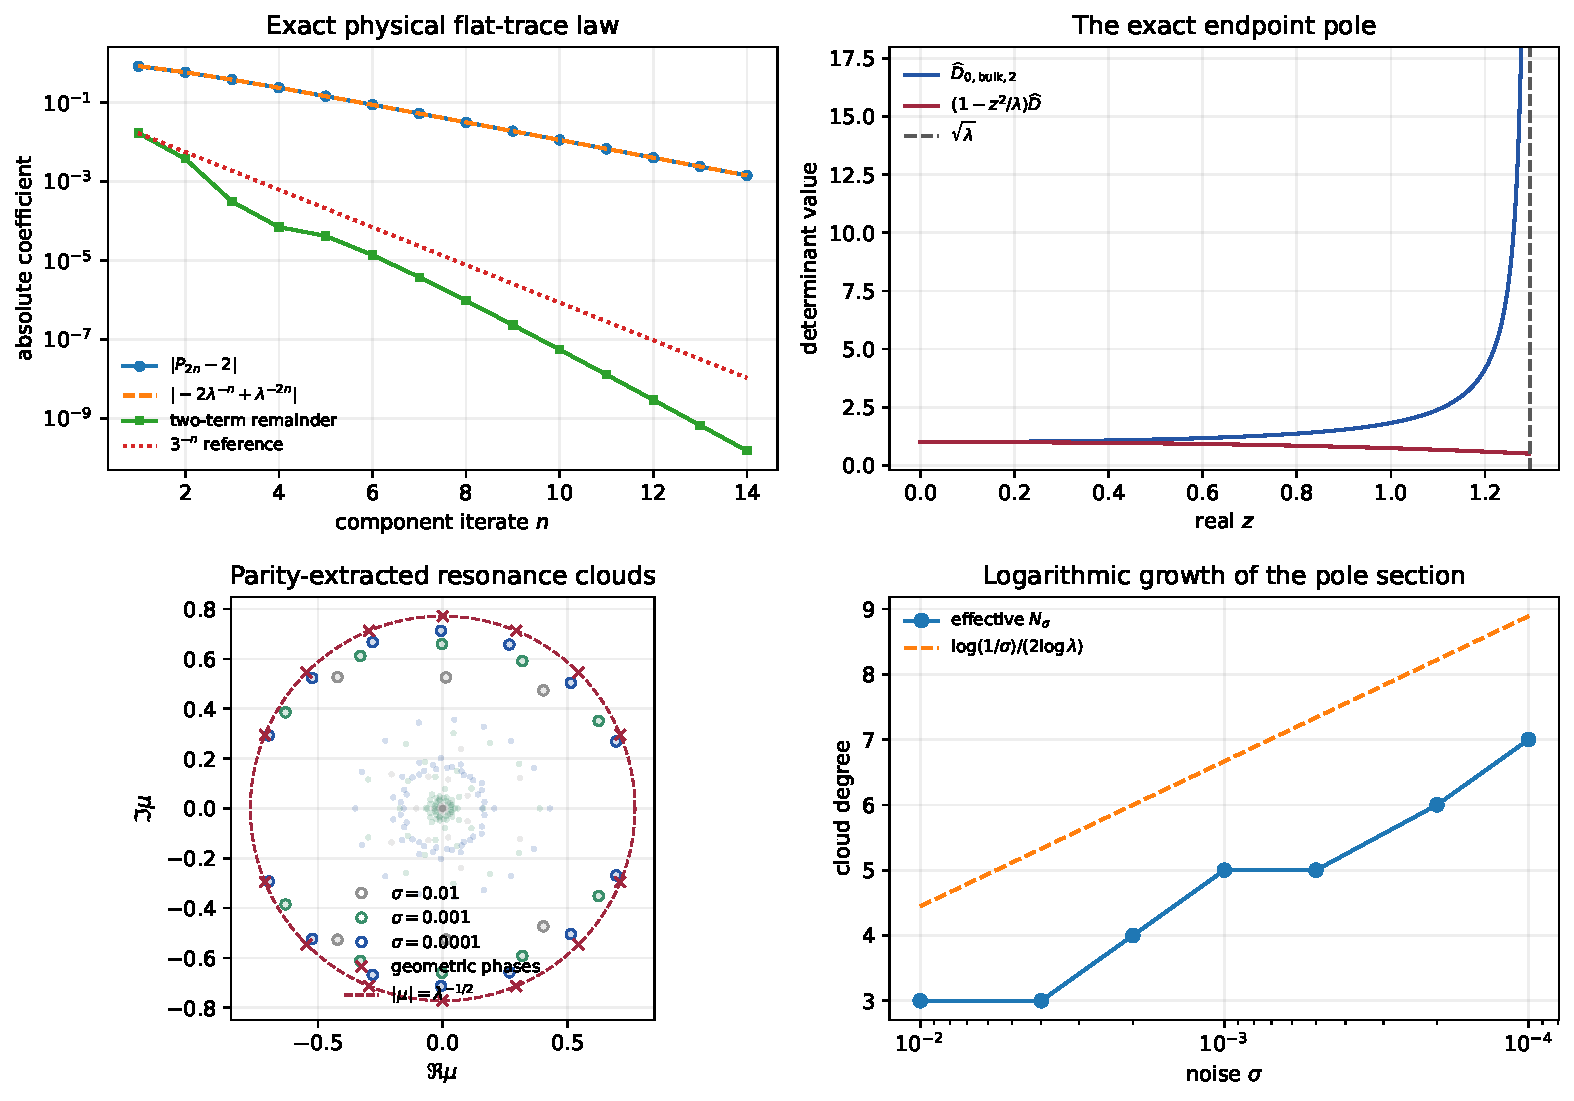
\includegraphics[width=\textwidth]{figures/exact_pole_resonance_cloud.pdf}
\caption{Exact target and noisy pole resolution.  Top left: the physical
centered trace and its two endpoint terms; the remaining reduced-sector
contribution decays faster.  Top right: the deterministic bulk determinant
diverges at $\sqrt\lambda$, while the pole-removed factor stays regular.
Bottom left: noisy bulk spectra after Perron/parity extraction; open circles
mark the selected clouds and crosses mark the $N=7$ geometric phases.  Bottom
right: the effective degree grows on the half-logarithmic localization
scale.}
\label{fig:pole-cloud}
\end{figure}

The tested cloud is stable under spatial refinement.  At $\sigma=0.001$,
changing $d\sigma$ from $10.24$ to $30.72$ leaves $N_\sigma=5$ at every
resolution.  The mean-radius spread is $1.87\times10^{-5}$, and the
bulk-radius spread is $1.50\times10^{-5}$.

\subsection{Radially centered scattering}

Let $\bar r_\sigma$ be the mean selected radius and let $C_\sigma$ be the
product over the selected conjugate cloud.  We evaluate the ratio in
\eqref{eq:noisy-scattering-conjecture} at
$s=-2,-1,-1/2,0,1/2,1,2$.  Radial centering is essential: at finite noise the
cloud lies inside its limiting circle, so centering directly at
$\sqrt\lambda$ mixes radial drift with phase scattering.

\begin{figure}[H]
\centering
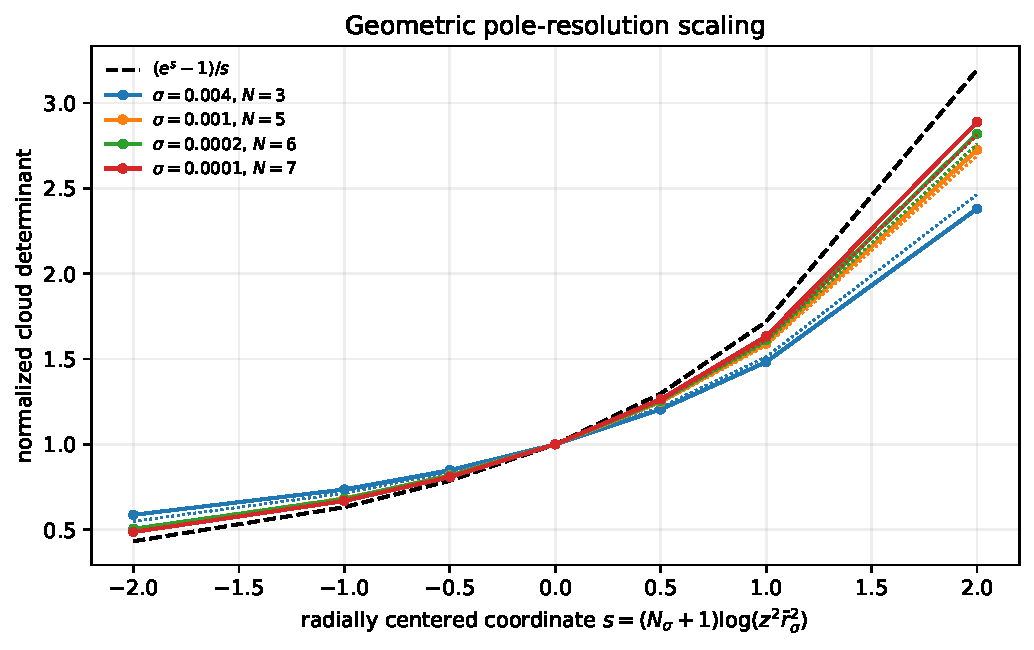
\includegraphics[width=0.82\textwidth]{figures/geometric_scattering_collapse.pdf}
\caption{Radially centered outer-cloud products.  Solid curves are the noisy
clouds, color-matched dotted curves are the exact finite geometric sections,
and the dashed curve is their $N\to\infty$ limit $(e^s-1)/s$.  The approach
to the universal curve is limited primarily by the small effective degrees.}
\label{fig:scattering}
\end{figure}

For $\sigma=10^{-4}$, the maximum discrepancy from the exact $N=7$ finite
section is $0.0198$ on $|s|\le1$ and $0.0761$ on $|s|\le2$.  This comparison
uses no phase or amplitude regression after the radial mean and the
automatically selected integer $N_\sigma$ are fixed.

\subsection{Approach inside the pole}

For determinant values, conjugate-complete ARPACK eigenpairs are multiplied
and the exactly computable second trace supplies a residual $m=2$
correction.  The deterministic comparison curve comes from
\eqref{eq:bulk-full-factorization}, not a periodic truncation.

\begin{figure}[H]
\centering
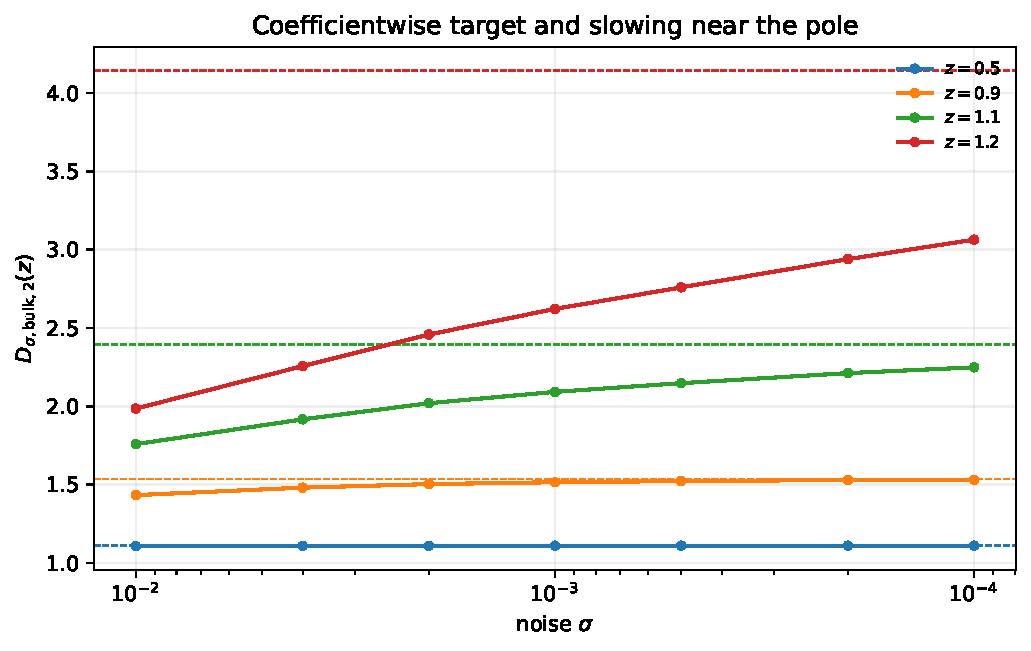
\includegraphics[width=0.82\textwidth]{figures/bulk_determinant_pole_approach.pdf}
\caption{Noisy bulk determinant diagnostics at fixed real targets.  Dashed
horizontal lines are the exact deterministic factorization.  Convergence is
clear well inside the pole and slows sharply as $z$ approaches
$\sqrt\lambda=1.2956\ldots$.}
\label{fig:determinant-convergence}
\end{figure}

At $\sigma=10^{-4}$ the absolute discrepancies are $2.49\times10^{-4}$ at
$z=0.5$, $4.85\times10^{-3}$ at $z=0.9$, and $1.08$ at $z=1.2$.
The last value is not evidence against coefficient convergence; it is the
expected nonuniformity near a pole whose effective section has degree only
seven.

\subsection{Numerical status}

All eigenvalues, cloud selections, phase errors, determinant values,
resolution checks, software versions, and source hashes are archived.  The
test suite checks the exact branch correction, reconstruction against the
independent physical periodic data, the reduced circle traces, geometric
zeros, scattering profile, synthetic cloud selection, row stochasticity, and
pole removal.

The sparse eigenvalues are ordinary double-precision calculations.  ARPACK
values near the 80-eigenvalue cutoff may omit one member of a nearly
degenerate pair; determinant diagnostics therefore retain only complete
conjugate pairs and correct the exact second trace.  The outer cloud is far
above that cutoff and is stable under spatial refinement.  None of these
computations is presented as interval validation.

\section{A proof route for noisy bulk scattering}
\label{sec:route-map}

The exact pole theorem narrows the remaining analysis to three operator
estimates.  Together they form a concrete route to
\cref{conj:noisy-scattering}.

\paragraph{1. Effective-rank control.}
The distinguished deterministic orbit approaches the state boundary at
distance $\asymp\lambda^{-m}$.  For the two-step component time $n=m/2$,
the equality $\lambda^{-2n}\asymp\sigma$ gives
\begin{equation}\label{eq:rank-clock}
 n\sim\frac{\log(1/\sigma)}{2\log\lambda}.
\end{equation}
A proof must turn this geometric horizon into upper and lower bounds
$N_\sigma=\log(1/\sigma)/(2\log\lambda)+O(1)$ for the dimension of the
endpoint transfer block.  This is a singular-value or approximation-number
problem, not another parity-eigenvalue calculation.

\paragraph{2. Shift-block reduction.}
After the two RH-14 boundary layers are extracted, the endpoint block should
be reduced by a Feshbach or Grushin map to a finite unilateral shift plus a
small remainder.  The characteristic polynomial of that shift is precisely
$\Pi_{N_\sigma}(z^2/\lambda)$.  Norm control of the remainder on the
$N_\sigma^{-1}$ spectral scale would prove both radial rigidity and the phase
grid in \eqref{eq:noisy-cloud-conjecture}.

\paragraph{3. Residual normality.}
Let $C_\sigma$ be the resulting cloud determinant.  One needs local bounds
for
\begin{equation}\label{eq:residual-family}
 \frac{D_{\sigma,\mathrm{bulk},2}(z)}{C_\sigma(z)}
\end{equation}
on compact subsets of $|z|<\lambda$.  Montel compactness and the exact Taylor
germ would then identify every subsequential limit with the nonzero factor
$\cG$.  This is exactly the estimate missing from coefficientwise
convergence.

These steps also specify falsification criteria.  If $N_\sigma$ does not obey
\eqref{eq:rank-clock}, if phase errors fail to shrink, or if the residual
family is not locally bounded, then the geometric scattering model is wrong
even though the deterministic pole theorem remains valid.

\section{Conclusion}

The parity-extracted determinant problem does not end in a conventional
entire small-noise limit.  The exact physical trace reconstruction shows why:
the deterministic bulk target has the noncanceled factor
\[
 \frac1{1-z^2/\lambda},
\]
and therefore two simple poles at $\pm\sqrt\lambda$.  This proves the sharp
physical coefficient law, rules out normal convergence through the first
spectral edge, and shows that finitely many limiting resonances cannot carry
the required negative moments.

Finite noise resolves the poles through a growing complex cloud.  At the
smallest computed noise, fourteen resonances lie near the radius
$\lambda^{-1/2}$ and the phases $\pm k\pi/8$.  After radial centering, their
determinant follows the exact geometric finite section whose scaling limit is
$(e^s-1)/s$.  The data therefore support a scattering continuation rather
than an eigenvalue-by-eigenvalue limit.

The next theorem is now sharply formulated: derive the logarithmic effective
rank, reduce the endpoint block to a finite shift, and prove normality after
cloud extraction.  No assertion about zeta zeros, Hilbert--P\'olya, or the
Riemann hypothesis is needed at this stage; the present result is an operator
and determinant statement at one explicit quadratic map.

\section*{Data and code availability}

The manuscript, source, tests, exact reconstruction tables, sparse spectra,
cloud selections, scattering data, determinant diagnostics, figures, and
machine-readable summary are archived with this paper
\citep{WangBulkScatteringCode2026}.

\bibliographystyle{plainnat}
\bibliography{references}

\end{document}
